%!TEX ROOT = thesis.tex
\chapter{Introduction, Background Story, Motivations}
\section{Basic Introduction}
%In the Introduction section, you should describe the problem investigated. Try to summarize relevant research to provide context, key terms, and concept so the reader can understand the whole final year project. Go and read journal or conference papers and review relevant past research to 
%provide rational or justification for your work. Define clearly your final project objectives and briefly describe your research – design, 
%research, hypothesis, etc.
Currently, the amount of vehicles on the road increases every year in Malaysia.  
It is because the local brand car is affordable by many low income level household. The manufacturer also provided promotions to attract people to buy car. So that, the number of non-professional driver rapidly increased in Malaysia. Most of the drivers are unskilled and lack of awareness on the traffic safety and vehicle condition. The driver's personal factors have become the main reason of causing the traffic incidents.

According to the general road accident data in Malaysia took from Malaysian Institute of Road Safety Research (MIROS) offcial website shown in Figure \ref{fig:accident}, the Malaysia government put effort on reducing the amount of traffic incidents by introducing the new traffic laws and speed track system. However, the number of cases of road deaths does not drop significantly. 

\begin{figure}[hbt!]\centering
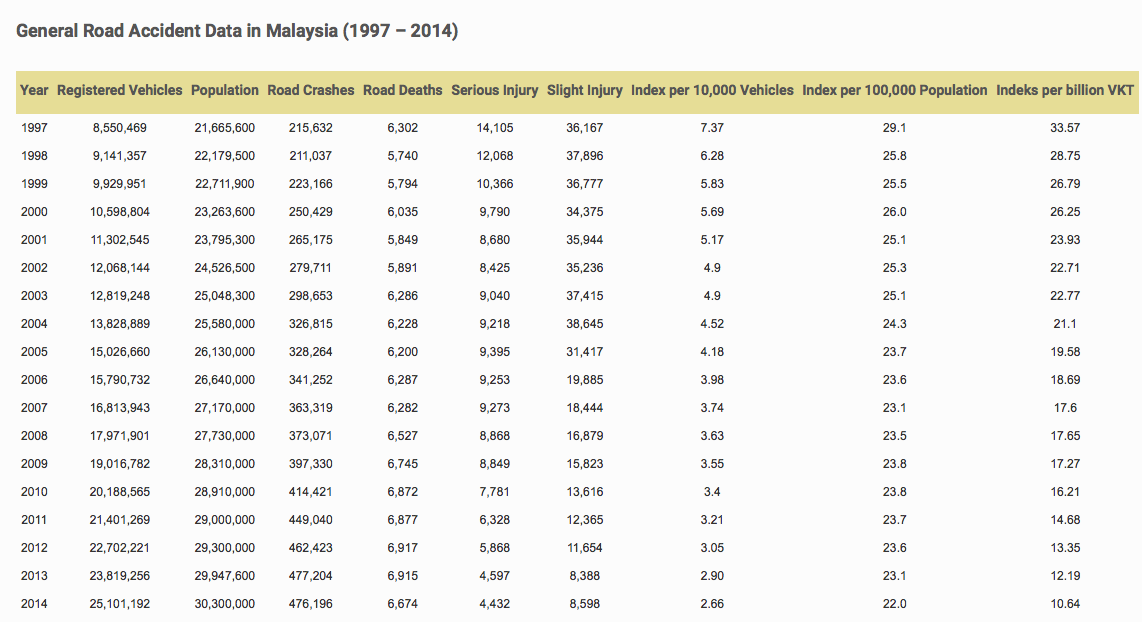
\includegraphics[width=.75\textwidth]{image/accident}
\caption{General Road Accident Data in Malaysia (1997 - 2014)}
\label{fig:accident}
\end{figure}

The driver characteristics and the occurence of traffic incident is interrelated. To further reduce the number of accidents, the safety equipment of the vehicle need to be improved as well as the road regulation, but also pay attention on driver behaviour. 

\subsection{Vehicle Operation Data Collection}
The behaviour of the driver is hard to be identified. The driver behavior is affected by environment, vehicle condition and the mental or physical state. One way to identify driver behaviour is using the vehicle operation data.

\subsubsection{OBD System}
The OBD system is also called OBD-II, was proposed in 1996. In 1996, all the cars manufactured in United State (US) were required to equip OBD-II and the cars without OBD-II prohibited to sell in US. The purpose to have OBD-II specifications is to diagnose engine problem. The specifications were being used by the Environment Protection Agency (EPA) and the state of California to meet the emission standards. Since 1996, all the cars in US are required to be equiped with OBD-II to establish the EPA regulation. 

The usage of the OBD-II is important for detecting the vehicle exhaustion. If the vehicle is exhaust high level of air-pollution content, Diagnostic Trouble Codes (DTCs) will be geneated by the OBD-II and a Check Engine Light will be displayed on vehicle dashboard. A OBD-II scanning tool can access the DTCs from the Engine Control Unit (ECU). 

\subsubsection{ELM327}
ELM327 is used in the data collection process. The ELM327 is a programed microcontroller. It is an interface to communicate with the On Board Diagnotics port of the vehicle. The ELM327 supports most of OBD-II protocols. ELM327 also contains the bluetooth adapter. The ELM327 needs to be plugged to the OBD-II port that can be found under the vehicle dashboard and above the pedals. 

\subsubsection{Torque(Lite)}
Torque Lite version is a free android application and it is able to be installed in smartphone from Google Play Store. The application will communicate with the ELM327 through the bluetooth connection. The application will collect the data received from the ELM327 and  save the data into a .csv file in the smartphone. 

\subsection{Driver Behavior Analysis}
Takahiro Wada, Shun'ichi Doi, Keisuke Imai, Hiroshi Kaneko, Naohiko Tsuru, and Kazuyoshi Isaji introduced a performance index for approach and alienation to analyze the drivers' behavior in longitudinal direction. The performance index is calculated based on the relative velocity and distance with the preceding car. The data is collected through a driver simulator. Based on the index, drivers' brake pattern can be analyzed.

\subsection{Driving Behavior Analysis Based on AdaBoost Algorithms}
Shi-Huang Chen, Jeng-Shyang Pan, and Kaixuan Lu proposed a driving behavior analysis based on AdaBoost Algorithms. The proposed method also based on vehicle OBD information. The proposed method colected the vehicle operation data, such as vehicle speed, engine speed, throttle position and engine load. The proposed method calculated the relative ratio of the vehicle speed and the engine speed, the relative ratio of the engine speed and throttle position, and engine load as three characteristics for the modeling usage. Then it uses the AdaBoost Algorithms to classify the driving behavior based on the three characteristics.

\section{Project Objective}
\begin{enumerate}
\item To identify the features that contribute to the accuracy of the classification of the driver behavior analysis from the vehicle operation data.
\item To profile the drivers based on the vehicle operation data. 
\end{enumerate}

\section{Research Motivation}
This project is designed to capture actual driving behavior data by using sensor. The driver behavior will be analysed based on the vehicle operation data collected from the sensor plugged in the particular vehicle.  
This project will use the ELM327 as a device that communicates with the vehicle OBD-II interface. The GPS data and vehicle operation data will be collected through the application Torque(Lite) via bluetooth. 
The performance index for approach and alienation will be used in this projetc as a feature to analyze the drivers' driving behaviour. The driver who exceed the speed limit can be detected by using the vehicle speed and the GPS location information.

\section{Project Scope}
This project focuses on the driver behavior profiling. The vehicle operation data will be collected and pre-processed before execute the analysis. The subjects are 10 adult drivers (2 female and 8 male) who owned the driving license at least two years. Each driver is required to drive the car at least 10 minutes for vehicle operation data collection. The data will be recorded in every second. For each driver, there are at least 600 records in the vehicle operation data file. After using the machine learning technique to classified the drivers, the drivers will be categorized to three classes. The classes are low risk, medium risk and high risk. 
 